\section{Project scheduling}

\begin{definition}[\textit{Task}]
    Tasks are activities that must be completed to achieve the project goal, also called work packages. 
\end{definition}
\begin{definition}[\textit{Milestone}]
    Milestones are points in the schedule in which you can assess progress. 
\end{definition}
\begin{definition}[\textit{Deliverable}]
    Deliverables are work products that are delivered to the customer. 
\end{definition}

Graphical notations are normally used to illustrate the project schedule
Gantt charts are the most commonly used representations for project schedules.
They show the schedule as activities or resources against time
Gantt diagrams often result from one or more of the following methods: 
\begin{itemize}
    \item \textit{Work breakdown structure}: details the work that must be done, breaks down the work into tasks that can be easy to estimate, assign and track. 
        \begin{figure}[H]
            \centering
            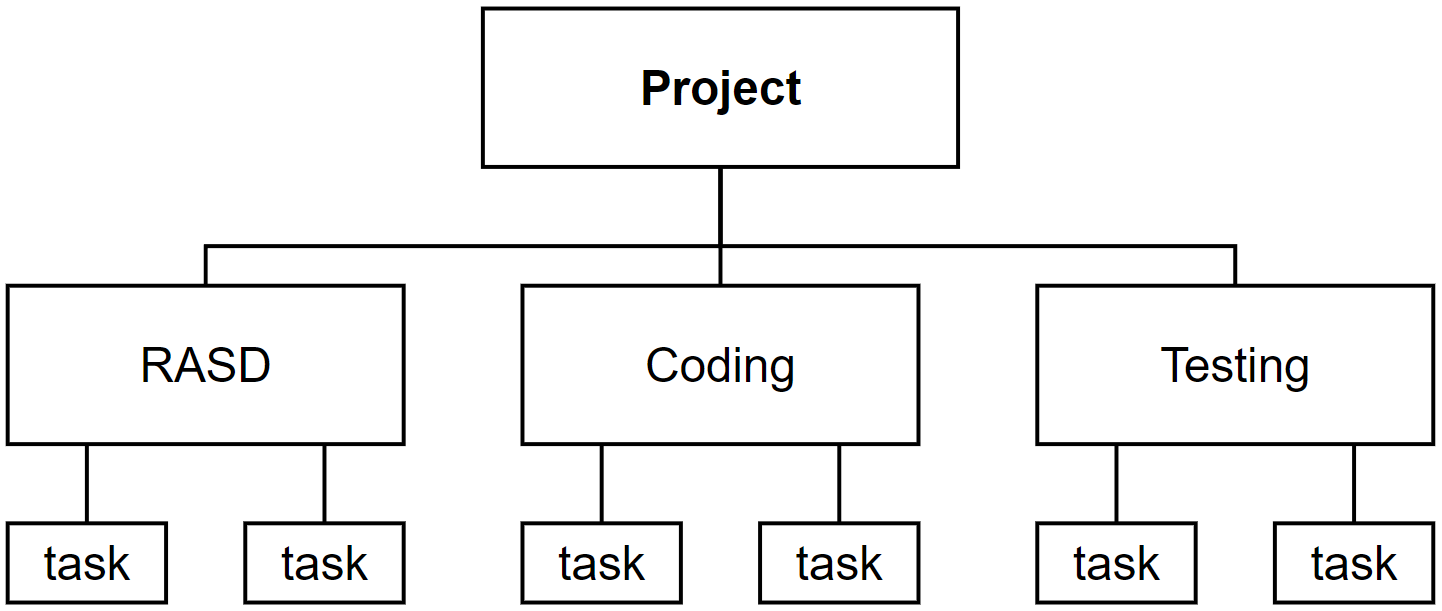
\includegraphics[width=0.5\linewidth]{images/wbs.png}
        \end{figure}
    \item \textit{Precedence diagram method}: technique used for constructing a schedule starting from the precedence relationships between activities. 
        In this phase we define which task (predecessor) triggers the other (successor) and introduce a delay with the LAG time (positive or negative). 
        \begin{figure}[H] 
            \centering
            \begin{minipage}[b]{0.4\linewidth}
                \centering
                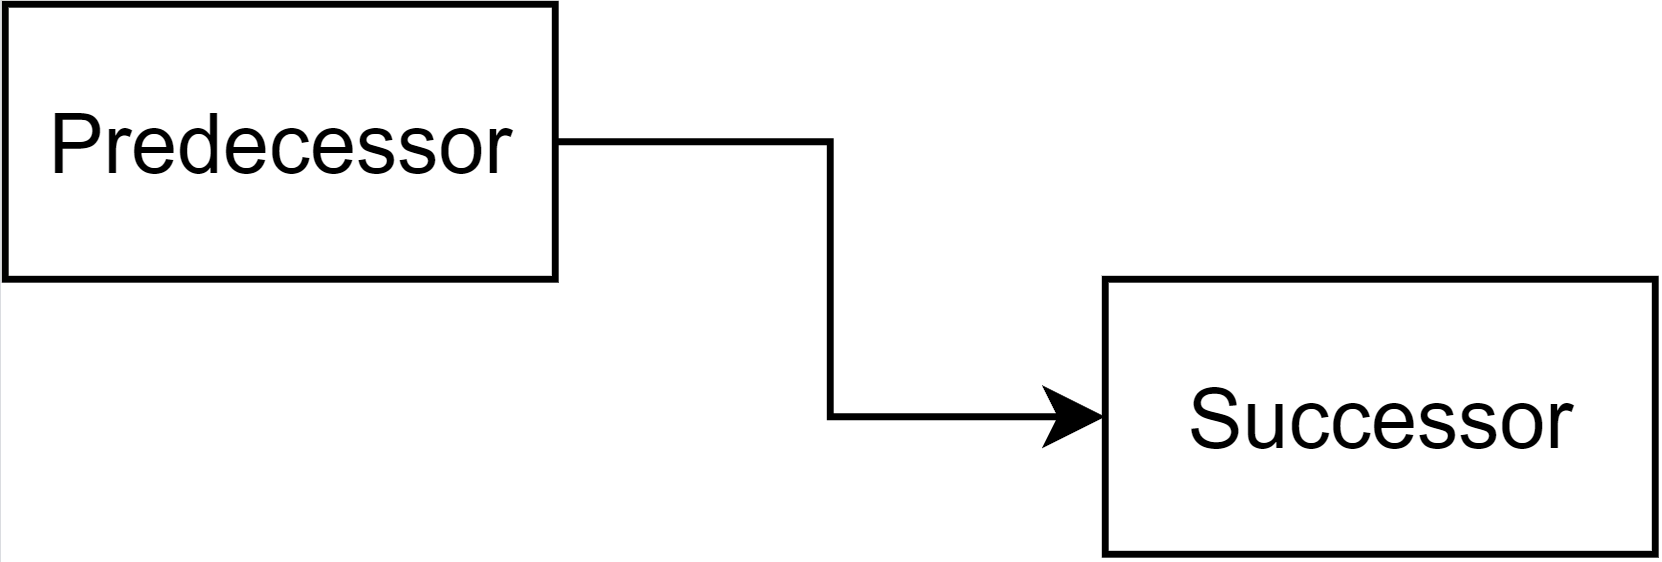
\includegraphics[width=0.9\linewidth]{images/fts.png} 
                \caption*{Finish to start} 
                \vspace{4ex}
            \end{minipage}%% 
            \begin{minipage}[b]{0.4\linewidth}
                \centering
                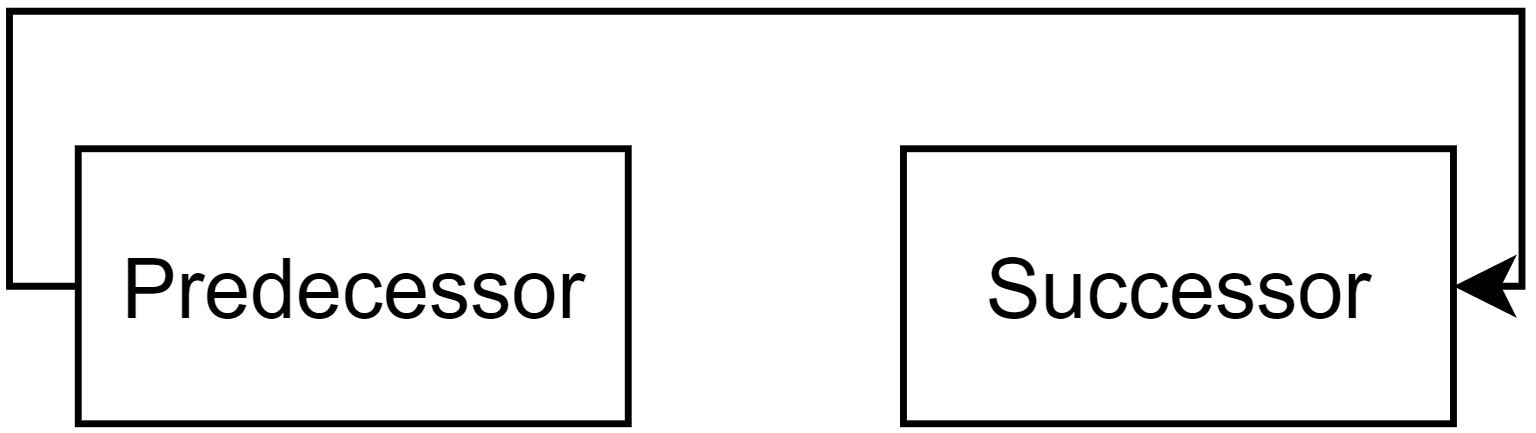
\includegraphics[width=0.9\linewidth]{images/stf.png} 
                \caption*{Start to finish} 
                \vspace{4ex}
            \end{minipage} 
            \begin{minipage}[b]{0.4\linewidth}
                \centering
                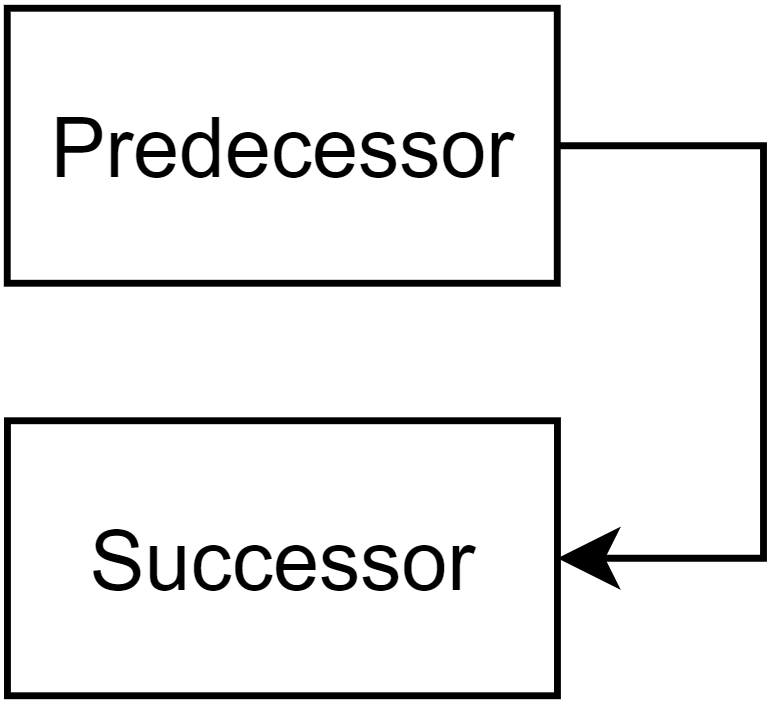
\includegraphics[width=0.4\linewidth]{images/ftf.png} 
                \caption*{Finish to finish} 
                \vspace{4ex}
            \end{minipage}%%
            \begin{minipage}[b]{0.4\linewidth}
                \centering
                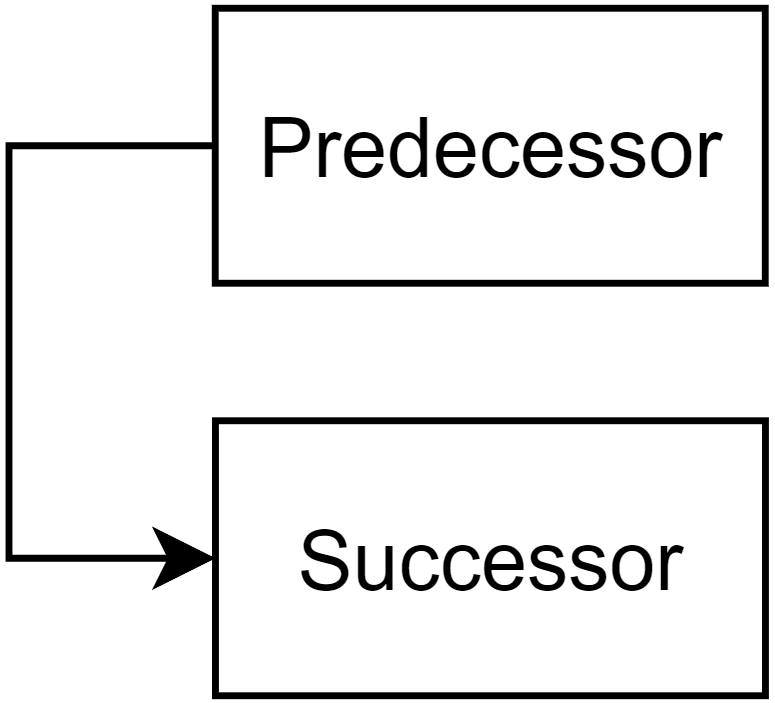
\includegraphics[width=0.4\linewidth]{images/sts.png} 
                \caption*{Start to start} 
                \vspace{4ex}
            \end{minipage} 
        \end{figure}
        Tasks and constraints in project scheduling can be categorized based on their flexibility:
        \begin{itemize}
            \item \textit{Flexible tasks}: these tasks are adaptable and can commence as soon as feasible.
            \item \textit{Partially flexible tasks}: these tasks bear some degree of flexibility, with the stipulation to start no earlier than a certain point and to conclude by a specified deadline.
            \item \textit{Inflexible tasks}: these tasks are rigid and must occur on a designated date, with no room for adjustments. 
                They have a strict start and finish schedule.
        \end{itemize}
    \item \textit{Critical path method}: the Critical Path Method (CPM) serves as a tool for approximating the minimum duration of a project. 
        By utilizing a project schedule network diagram and activity duration estimates, it calculates crucial parameters such as early start, early finish, late start, and late finish dates. 
        These calculations are made to ensure that the project finish date and any specified schedule constraints remain unaltered.
        Task float, representing the difference to the finish date, is a key metric. 
        A task is deemed critical if its float is zero, signifying that any delay would impact the project timeline. 
        The critical path, consequently, forms a continuous sequence of tasks extending from the project's commencement to its conclusion. 
        Importantly, any modifications to tasks along the critical path directly influence the project's finish date.
\end{itemize}





















